\documentclass{article}
\usepackage[utf8]{inputenc}
\usepackage{amsmath}
\usepackage{graphicx}
\usepackage[parfill]{parskip}
\usepackage{fancyhdr}

\usepackage{biblatex}
\usepackage{booktabs}

\usepackage[utf8]{inputenc}
\usepackage[T1]{fontenc}
\usepackage[ngerman,english]{babel}
\usepackage{tabularx}  % for 'tabularx' environment and 'X' column type
\usepackage{ragged2e}  % for '\RaggedRight' macro (allows hyphenation)
\newcolumntype{Y}{>{\RaggedRight\arraybackslash}X} 
\usepackage{booktabs}  % for \toprule, \midrule, and \bottomrule macros 
\usepackage{hyperref}

\usepackage[all]{hypcap}

\addbibresource{ref.bib}


\renewcommand{\figurename}{Figur}
\renewcommand{\tablename}{Tabell}


\begin{document}
\pagenumbering{gobble}
\newcommand{\HRule}{\rule{\linewidth}{0.5mm}}

\begin{center}

\textsc{\LARGE NTNU}\\[1.5cm] 
\textsc{\Large TTK4235}\\[0.5cm]
\textsc{\large Labgruppe 30}\\[0.5cm]

\HRule \\[0.4cm]
{ \huge \bfseries Rapport heislab}\\[0.4cm]
\HRule \\[1.5cm]
 
\begin{minipage}{0.6\textwidth}
\begin{flushleft} \large
\emph{Authors:}\\
Thomas \textsc{Borge Skøien} \\Vegard \textsc{Haraldstad} \\
\end{flushleft}
\end{minipage}
~
\\[1cm]

{\large \today}\\[1cm] 

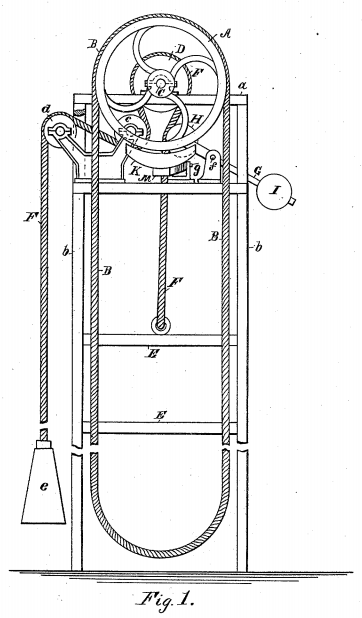
\includegraphics[height=80mm]{rapport/heis.PNG}

\end{center}
\newpage
\cfoot{\normalsize\thepage}
\pagenumbering{roman}

\tableofcontents


\newpage
\nocite{*}
\cfoot{\normalsize\thepage~}
\pagenumbering{arabic}
\section{Overordnet arkitektur}

Den overordnede arkitekturen vår gikk ut på å lage simple moduler, med en kontrollenhet som tar seg mer av den finjusterte logikken. Dette gjorde at modulene forutenom kontrollenheten kunne bli produsert i parallell. Elevator skulle bli vårt grensesnitt mot hardware, mens queue skulle ta seg av å si ifra hvilken bestilling som vil være neste i vår gitte retning. Dette gjorde at vi kunne gjøre all høynivå logikk som retning på heisen, og states i control, mens neste etasje logikken ble alt gjort i queue, slik at control ikke hadde behov får å se den faktiske køen. Vi tok også et valg ved å gjøre queue avhengig av hardware. Dette var noe vi ikke gjorde i starten men noe vi bestemte oss for underveis. Slik vi satte opp programmet, ble det fornuftig å ta seg av all lysbehandling i queue, slik at vi kunne garantere at alle lysene alltid var satt riktig, ved at queue hadde en tett sammenheng mellom hva som lå i queue, og hva den gjorde med lysene. På denne måten ungikk vi også en egen lysmodul eller lignende, og vi slapp også mye logikk i kontroll for å sende dette videre til elevator, som allerede ble en stor nok modul som tok seg av bevegelse. Control var da ikke direkte avhengig av hardware, og var et abstraksjonsnivå over elevator og queue, ved at disse ble grensesnittene til kontrollmodulen. Vi lagde også en timermodul som inneholdt en universell timer for hele heisen.

\begin{figure}[h!]
  \centering
  \advance\leftskip-0.6cm
  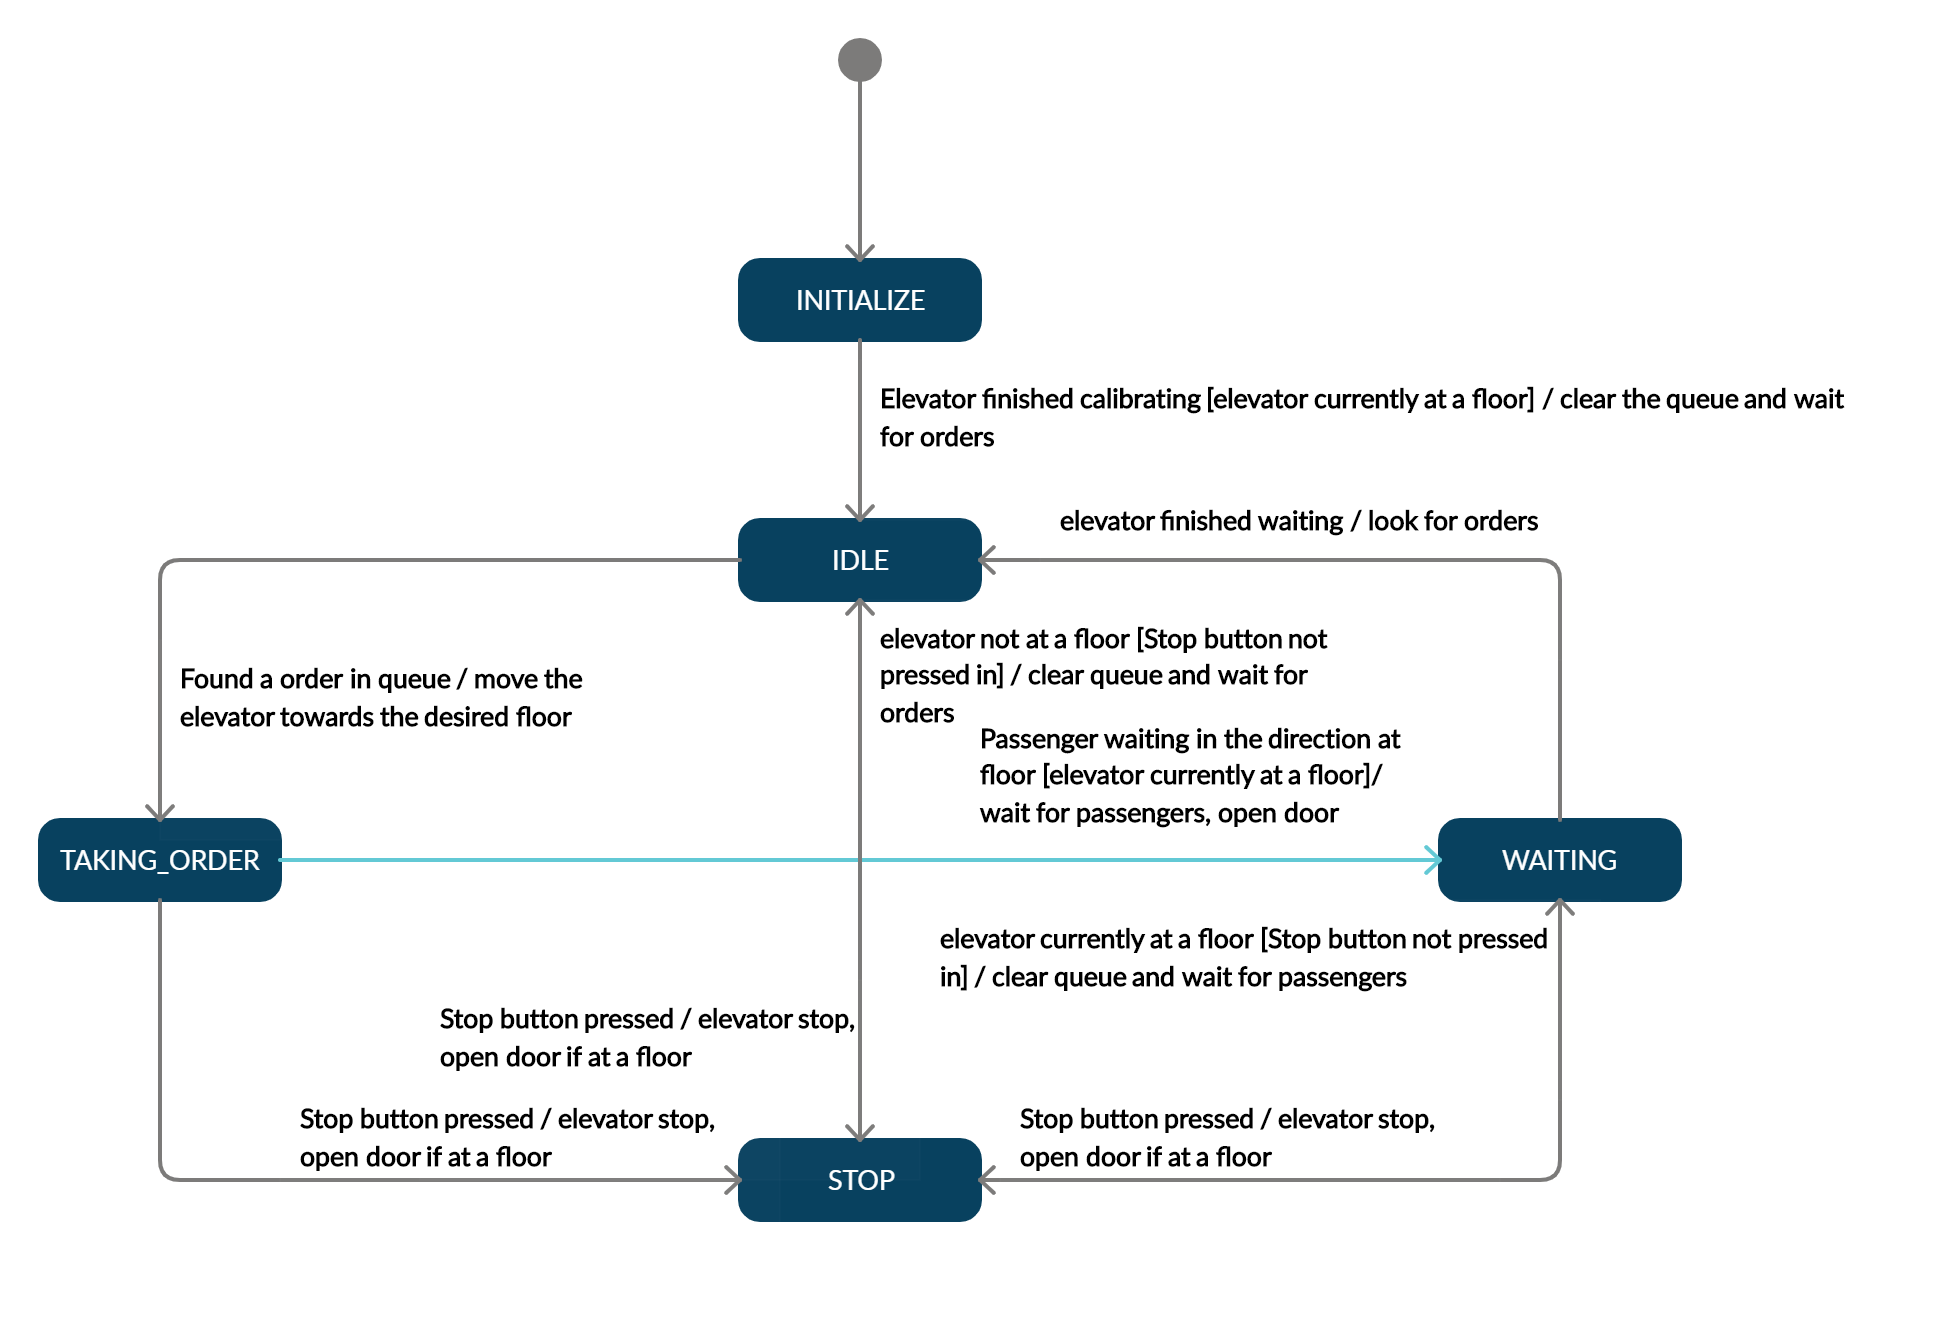
\includegraphics[width=450]{rapport/State_elevator_diagram.png}
  \caption{Tilstandsdiagram}
  \label{fig:StateDia}
\end{figure}

Ved å ta de valgene vi har tatt vil vi si at vi er ganske sikre på at heisen vår tilfredsstiller kravspesifikasjonen. Selv om det kan måtte bli ekstra bry for å skrive om modulene dersom grensesnittet til hardware endres, så vil dette garantere med stor sannsynlighet at lysene blir satt riktig, og at det dermed var lurt for vår arkitektur å ha en avhengighet mellom queue og hardware. Dette gjorde også at testingen ble enklere, ved at lysene kunne bli en visuell representasjon av køen, ettersom disse gjenspeilet hverandre, og det ble enklere å se hvor feilen faktisk lå. Under designet av arkitekturen la vi vekt på å følge kravspesifikasjonen så enkelt som mulig, ved å ha få velfungerende moduler som en kan se i klassediagrammet på figur \ref{fig:KlasseDia}. Queuemodulen sin kø, ble laget ved et simpelt array, noe som gjorde at logikken ble enkel, og vi unngår problemet med å kunne ende opp med minnelekasje. Dette gjorde at det ble enkelt å gjøre endringer i controlmodulen underveis. Dersom det oppsto en bug var det få steder å feilsøke, og med få states i vår tilstandsmaskin, unngikk vi å overkomplisere heisen. Vi fikk abstrahert bort i ulike en høynivå og to lavere nivå moduler, dette ser vi godt i sekvensdiagrammet i figur \ref{fig:sekvensdi} der grensesnittet fra kontroll til de andre enhetene er ganske lite, og mye blir abstrahert bort. Dette vil også gjøre det enklere å omprogrammere heisen om et nytt køsystem skal legges til. I tilstandsdiagrammet i figur \ref{fig:StateDia} ser vi også de få tilstanden til tilstandsmaskinen, og hvor enkelt det er å komme fra og til stopp, slik at sikkerheten ligger først i vårt system.

\begin{figure}[hp]
  \centering
  \advance\leftskip-1cm
  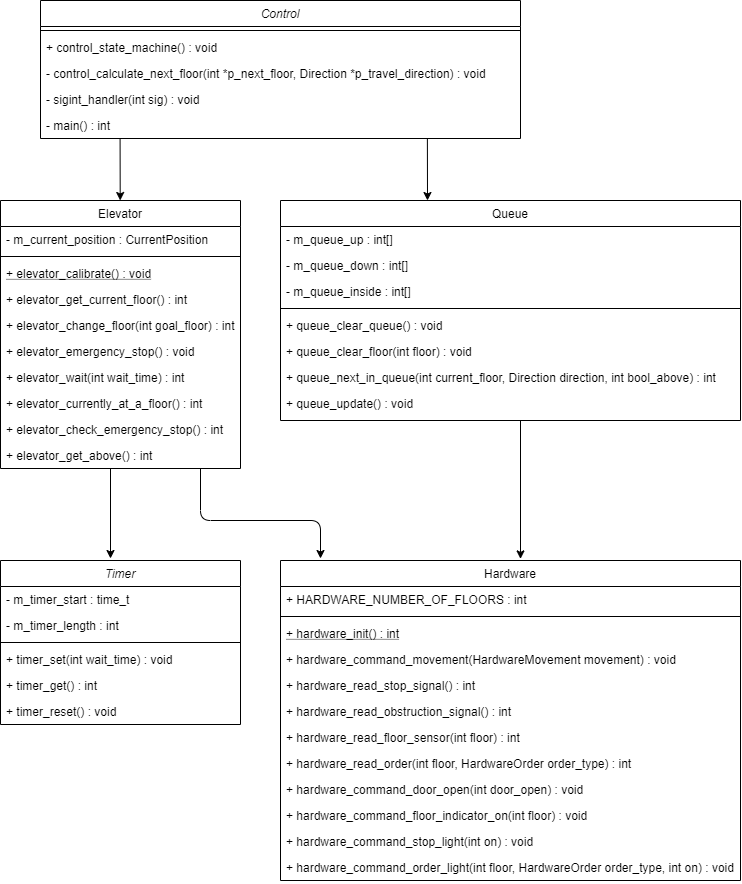
\includegraphics[width=430]{rapport/klassediagram.png}
  \caption{Klassediagram}
  \label{fig:KlasseDia}
\end{figure}

\begin{figure}[hp]
    \centering
  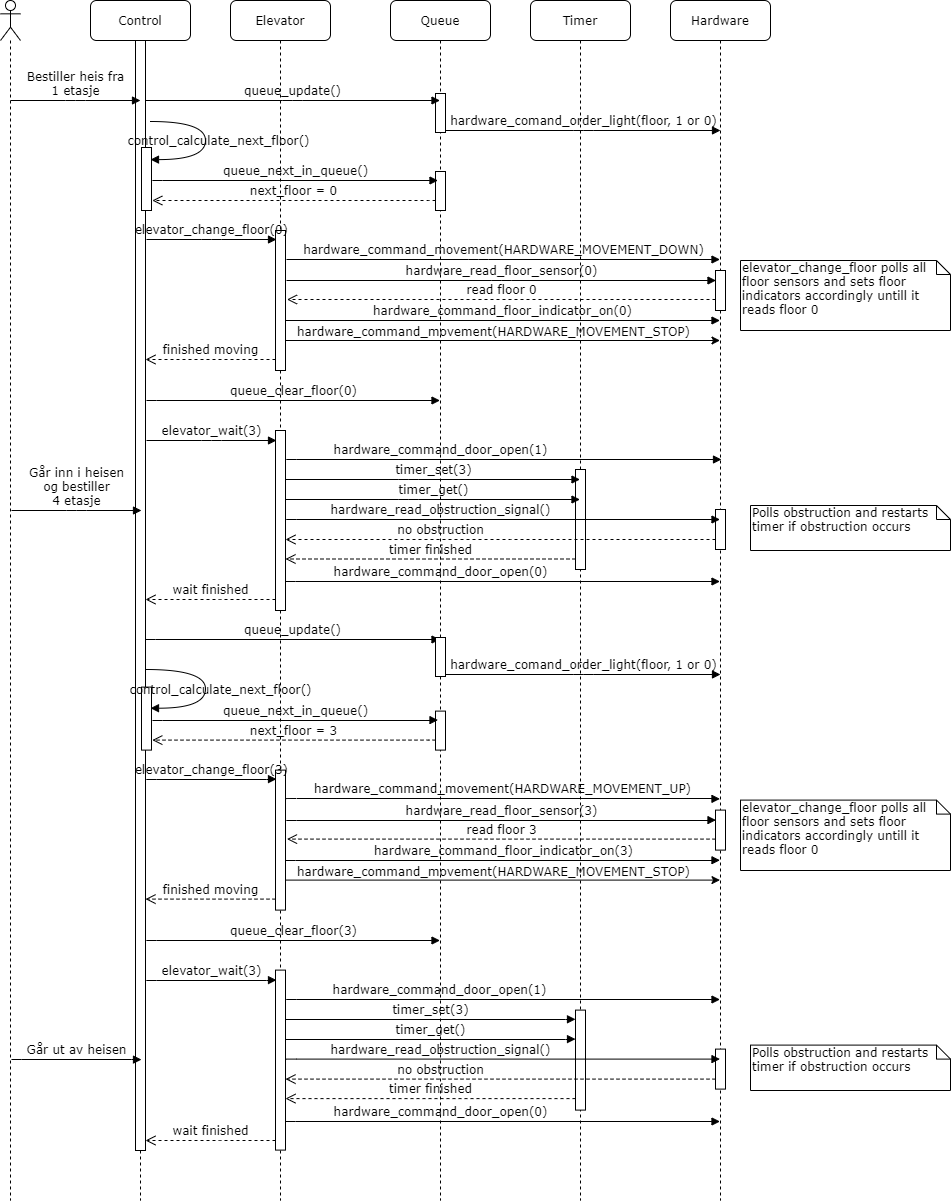
\includegraphics[height=\textheight]{rapport/Sekvensdiagram.png}
  \caption{Sekvensdiagram}
  \label{fig:sekvensdi}
\end{figure}

\section{Moduldesign}
\subsection{Control}
Controlmodulen vår er det øverste laget i arkitekturen vår og tar seg av mesteparten av beslutningstagningen. Logikken ble implementert som en tilstandsmaskin med 5 tilstander. Dette er en høynivå modul og har ingen direkte tilknytning til hardware. Det er også i denne modulen main() funksjonen ligger, og er kjernen i programmet. I utgangspunktet hadde vi bare 4 tilstander, men vi la til waiting, for å skille ut dørfunksjonen, gjøre logikken enklere og tryggere for feil. Tryggere for feil fordi all dørfunksjonalitet ble lagt i en tilstand, der den måtte komme inn i denne tilstanden for at døren skulle kunne åpne seg.  Dette gjorde også at stopp funksjonaliteten også ble enklere, ved at om stopp knappen slippes i en etasje, kan vi gå rett til waiting.
\subsection{Queue}  
Kømodulen vår ble designet med mål om å være enkel, noe som igjen førte til at veldig lite av beslutningstagningen blir gjort i queue. Selve køen er implementert som tre arrays av ints, en for bestillinger opp, en for ned og en for bestillinger fra heisvognen. Hvert element i arrayene representerer hvovidt vi har en bestilling i en gitt etasje, av typen arrayet representer, eller ikke. Med denne typen implementasjon ønsket vi videre at køen og bestillingslysene på betjeningsboksen skulle speile hverandre. På denne måten ble setting av bestillingslys veldig enkelt og selv om det gir en sterkere kobling mellom queue- og hardwaremodulen anså vi det som fordelaktig med en slik implementasjon da grensesnittet til queue blir veldig enkelt og mulighet for feil i setting av bestillingslys er veldig liten. Det beste hadde klart vært å hatt et køsystem som var uavhengig av hardware med tanke på testing, men da queue ikke er avhengig av noen returverdier fra hardware kan queue likevel ganske enkelt testes isolert ved å kommentere ut alle funksjonskall til hardwarefunksjoner. Man kan også bruke bestillingslysene som en fysisk representasjon av køen under integrasjonstestingen, som igjen gjør det lettere å oppdage feil i forbindelse med køen.
\subsection{Elevator}
Elevator er designet som en modul som tar flere av de sekvensielle funksjonene man ønsker en heis skal ha og wrapper dem til et enkel grensesnitt som kan brukes av control. Eksempler på slike funksjoner er å la heisen endre etasje, la heisen åpne dørene eller kalibrering av heisen. Dette gjør at control ikke trenger å oppdatere hvor den er, eller hvordan den skal komme seg til en etasje, den bare spør etter hvor den er, sier hvor den skal, så tar elevator av seg resten. Elevator har dermed også da full kontroll på sin posisjon, både i og mellom etasjer. Denne modulen gjør om de vanlige funksjonen til en heis om til funksjoner som kan kalles, slik at en annen utvikler enklere kan bruke heisen, i stedet for å måtte tenke på hardware.
\subsection{Timer}
Timermodulen vår tar seg av timeren som brukes til å holde heisdøren oppe et visst antall sekunder. Den baserer seg på det innebygde biblioteket time, der vi lagret tiden som sekunder siden 1970. Dette gjør at heisen skal kunne kjøres i langt tid, uten å måtte startes på nytt. Slik modulen vår er satt opp er det bare en timer som kan settes om gangen. Så sekvensielt som programmet vårt er, og siden det aldri skal settes flere timere samtidig, var ikke dette et problem. Det gjorde også grensesnittet enklere mot de andre modulene, ettersom de ikke trenger å huske tiden. 
\section{Testing}
\subsection{Modultesting}
Timermodulen vår ble testet ved å skrive et enkelt testprogram som satte timeren, pollet den og avsluttet når timeren hadde gått ut, på samme måte som timeren blir brukt i det ferdige programmet. Queuemodulen vår ble også testet ved å skrive et testprogram som brukte funksjonene for å legge til og fjerne bestillinger, samt funksjonen for å slette alle bestillinger, mens man hele tiden overvåket den faktiske køen og så at den oppdaterte seg som ønsket. I tillegg ble funksjonen som retunerer neste etasje i køen testet på samme måte. Elevatormodulen ble også testet ved å skrive et testprogram, for deretter å observere om heisen vår gjorde som den fikk beskjed om. Her var det å gå inn i GDB, endre verdiene som ble sendt til elevator\_change\_floor funksjonen, og observere mens heisen bevegde på seg.
\subsection{Integrasjonstesting}
Integrasjonstestingen ble i stor grad en testing av controlmodulen, i og med at den syr sammen de andre modulene våre. Her var det å gå inn på alle testene vi hadde skrevet ned på forhånd, og sjekke om de funket en etter en. Kontrollmodulen måtte bli skrevet om underveis for å kunne bli sydd sammen med de andre modulene ettersom den var avhengig av både queue og elevator. Her fulgte vi V-modellen, gjorde en test, sjekket om det funket, endret på logikken, og gikk tilbake for å teste.
\subsection{Testprosedyre}
Testprosedyren vår er besert på kravspesifikasjonen i oppgaven og skal sikre at heisen vår består FATen. Etter at vi hadde en heis som oppfylte testprosedyren vår valgte vi å legge vekt på robustheten av systemet og testet derfor flere edge-cases for å fremprovosere feil. Når en edge-case hadde blitt rettet testet vi først edge-casen vi forsøkte å løse. Hvis dette fungerte som ønsket gjentok vi testprosedyren for å sikre at vi fortsatt oppfylte de generelle testene våre. 

\newpage
\subsubsection{Oppstart}

\begin{table}[htbp]
\begin{tabularx}{\textwidth}{ l l }  % use 'Y' for first column
\toprule
Punkt & Test \\
        \midrule
        \textbf{O1} & Start heis mellom to etasjer og sjekk at heis kommer i definert \\
        & tilstand. Start en gang til mellom to etasjer og trykk på \\
        & stoppknappen under kalibrering. \\
        \midrule
        \textbf{O2} & Start heis mellom to etasjer og forsøk å bestille etasjer. Ingen \\ 
        & bestillinger skal bli gjort før heisen er kalibrert. \\
        \midrule
        \textbf{O3} & Trenger ikke å teste out of bounds scenario. \\
\bottomrule
\end{tabularx}
\label{table:nonlin}
\end{table}

\subsubsection{Håndtering av bestillinger}
\begin{table}[htbp]
\begin{tabularx}{\textwidth}{ l l }  % use 'Y' for first column
\toprule
Punkt & Test \\
        \midrule
        \textbf{H1} &Trykk inn tilfeldige sekvenser av bestillinger flere ganger og påse at \\
        & alle bestillinger blir utført i riktig rekkefølge. Neste sekvens trykkes \\
        & inn før heis har utført alle bestillinger fra forrige sekvens. \\
        & Ulike sekvenser trykkes inn minimum tre ganger og frem til alle \\
        & bestillinger er gjort minst en gang. \\
        \midrule
        \textbf{H2} & Start i 1. etg og bestill 4. etg, 2. etg ned og 3. etg ned. Heis skal \\
        & ikke stoppe i 2. og 3. etg på vei opp. Utfør samme test i \\
        & motsatt retning. \\
        \midrule
        \textbf{H3} & Stoppe i alle etasjer. Sjekk at bestillinger tilhørende etasjen blir\\
        & fjernet. \\
        \midrule
        \textbf{H4} & Trykk 3 tilfeldige sekvenser av bestillinger og se at heis står i ro \\
        & etter at bestillinger er utført. \\
\bottomrule
\end{tabularx}
\label{table:nonlin}
\end{table}
\newpage
\subsubsection{Bestillingslys og etasjelys}
\begin{table}[htpb]
\begin{tabularx}{\textwidth}{ l l }  % use 'Y' for first column
\toprule
Punkt & Test \\
        \midrule
        \textbf{L1} & Gjør et utvalg bestillinger, se at hver gang heisen\\
        & stopper i en etasje så slettes alle bestillingslys i den etasjen. \\
        \midrule
        \textbf{L2} & Arkitekturen vår tilsier at dersom det ikke er noe i queuen, har \\
        & queuen tatt seg av å slette bestillingslyset også. Sjekk at dette \\
        & stemmer under vanlig kjøring. \\
        \midrule
        \textbf{L3} & Kjør heisen fra 1 til 4, sjekk at etasjelysene oppdateres kontinuerlig \\
        & oppover, gjør så det samme ned til 1 etasje\\
        \midrule
        \textbf{L4} & Jamfør forrige punkt. \\
        \midrule
        \textbf{L5} & Dette kommer fra hardware, og er alltid exclusive. \\
        \midrule
        \textbf{L6} & For alle de ulike tilstandene: ta en ordre, stå stille, venter på  \\
        & passasjerer, kalibrerer og stopp; sjekk at stoppknappen lyser når  \\
        & den holdes inne, og slutter når den slippes. \\
\bottomrule
\end{tabularx}
\label{table:nonlin}
\end{table}

\subsubsection{Døren}
\begin{table}[htbp]
\begin{tabularx}{\textwidth}{ l l }  % use 'Y' for first column
\toprule
Punkt & Test \\
        \midrule
        \textbf{D1} & Send heisen til en tilfeldig etasje, sjekk at heisen stopper i etasjen\\
        & og at døren åpnes i 3 sekunder. \\
        \midrule
        \textbf{D2} & Stopp heisen i og utenfor etasjer. Da skal bestillingene være slettet, \\
        & og døren skal aldri åpnes dersom den er utenfor en etasje. \\
        \midrule
        \textbf{D3} & Aktiver stoppknappen når heisen står stille i en etasje, og når den\\
        & er på vei forbi en etasje den ikke skal stoppe i. I begge tilfeller skal \\
        & heisen stoppe. Etter at døren åpnes, prøv å slipp stoppknappen for \\
        & så å trykke den inn igjen. Sjekk at døren holdes åpen. Til slutt slipp \\
        & stoppknappen og sjekk at det tar 3 sekunder før døren lukkes. Dette \\
        & punktet bør kombineres med D4.\\
        \midrule
        \textbf{D4} & Stopp i en etasje, aktiver obstruksjonsbryteren, sjekk at døren \\
        & ikke lukkes, skru så obstruksjonsbryteren av og på noen ganger. \\
        &  Sjekk at døren fortsatt ikke lukkes. Så skru av obstruksjonsbryteren \\
        & og sjekk at det tar 3 sekunder før døren lukkes igjen \\
\bottomrule
\end{tabularx}
\label{table:nonlin}
\end{table}
\newpage
\subsubsection{Sikkerhet}
\begin{table}[htbp]
\begin{tabularx}{\textwidth}{ l l }  % use 'Y' for first column
\toprule
Punkt & Test \\
        \midrule
        \textbf{S1} & Under normal testing, sjekk at dørlyset aldri lyser når heisen beveger \\
        & seg. \\
        \midrule
        \textbf{S2} & Kjør heisen mellom to etasjer og trykk stoppknappen. Prøv så å gå \\
        & til forrige etasje, for så å trykke på stopp igjen. Veksle mellom opp \\
        & og ned, sammen med stopp for å sjekke at dørene aldri åpner seg når \\
        & den befinner seg mellom to etasjer.\\
        \midrule
        \textbf{S3} & Dette punktet vil være oppfyllt dersom de andre testene er oppfyllt.\\
        & Under testing, sjekk at next\_floor aldri blir satt til en verdi som er\\
        & utenfor heisrommet, da vil den heller aldri gå utenfor. \\
        \midrule
        \textbf{S4} & Aktiver stoppknappen i og utenfor en etasje, sjekk at heisen stopper\\
        & med en gang.\\
        \midrule
        \textbf{S5} & Aktiver stoppknappen i og utenfor en etasje, sjekk at queuen slettes.\\
        \midrule
        \textbf{S6} & Aktiver stoppknappen, og hold den inne, både i og utenfor en etasje,\\
        & prøv så alle mulige bestillinger og sjekk at ingen blir lagret i queue. \\
        \midrule
        \textbf{S7} & Stopp heisen mellom to etasjer, sjekk at den står i ro. Stopp så \\
        & heisen i etasjene, og sjekk at den fortsatt står i ro. \\
\bottomrule
\end{tabularx}
\label{table:nonlin}
\end{table}

\subsubsection{Robusthet}
\begin{table}[htbp]
\begin{tabularx}{\textwidth}{ l l }  % use 'Y' for first column
\toprule
Punkt & Test \\
        \midrule
        \textbf{R1} & La heisen bevege seg fra en gitt etasje og aktiver så \\
        & obstruksjonsbryteren. Prøv stopp knapp, og generelle bestillinger og \\
        & sjekk at alt går igjennom. \\
        \midrule
        \textbf{R2} & Under testingen, la programmet kjøre mellom hver test, dersom \\
        & udefinert oppførsel oppstår, prøv å reproduser det. \\
        \midrule
        \textbf{R3} & Kjør heisen som normalt opp og ned mellom alle etasjene. Gå i \\
        & GDB og sjekk posisjonen til heisen, sjekk at både current floor \\
        & og above er satt til riktig verdi uansett posisjon, da vet den alltid \\
        & hvor den er. \\
\bottomrule
\end{tabularx}
\label{table:nonlin}
\end{table}
\newpage
\subsubsection{Ymse}
\begin{table}[htbp]
\begin{tabularx}{\textwidth}{ l l }  % use 'Y' for first column
\toprule
Punkt & Test \\
        \midrule
        \textbf{Y1} & Under normal testing, påse at heisen oppfører seg som normalt,\\
        & dersom den ikke gjør det, reproduser det og fiks det. \\
\bottomrule
\end{tabularx}
\label{table:nonlin}
\end{table}

\section{Diskusjon}
En av svakhetene som er viktige å diskutere i vårt arkitekturvalg er nødvendigvis valget av å gjøre queuemodulen avhengig av hardware. Problemet med å gjøre queue avhengig av hardware er at modultestingen blir mer kronglete. Likevel kan det argumenteres for at setting av etasjelys ble så enkelt nettopp på grunn av at vi valgte å gjøre dette i queue. Skulle vi for eksempel ha tatt hånd om etasjelysene i control hadde vi mistet det klare skillet i abstraksjonsnivå vi ønsker og hadde vi gjort det i elevator hadde det blitt avhengigheter på tvers av abstraksjonsnivåene, samt at det er en god kilde til å innføre bugs der bestillingslysene ikke gjenspeiler de faktiske bestillingene i systemet. Samtidig blir grensesnittet til queue veldig lite og dermed bruken i control enkel. 

Vi kom også frem til at timermodulen vår kunne ha en type svakhet i det at den bare teller heltallsekunder. Denne betyr i praksis at hver gang timeren aktiveres gjøres det med en viss usikkerhet, det blir aldri nøyaktig 3 sekunder åpningstid for eksempel, men i gjennomsnitt vil det jo bli det. Dersom det er viktig at det er nøyaktig 3 sekunder åpning hver gang, ville det blitt nødvendig å skrive om tidsbiblioteket til å for eksempel bruke millisekunder istedenfor.

Vi valgte også underveis å legge litt mer logikk inn i queue, enn i control. Litt for å gjøre queue litt mer intuitiv, slik at vi slapp å kalle queue med merkelige kall for å få det resultatet vi ønsket. For eksempel, hadde vi i starten mye av logikken i control, slik at vi måtte kalle queue, som om vi var i en annen etasje enn den vi var for å få ønsket resultat, dermed endte vi opp med å skrive om queue, for å få et litt enklere grensesnitt.

Vi valgte også å gå for et par get-funksjoner i elevatormodulen, dette for å holde abstraksjonsnivåene ulike i de ulike modulene. Istedenfor dette kunne vi sendt variable som referanser til de ulike elevatorfunksjonene. Det kan sies at vi prøver å tvinge en viss objektorientert programmering inn i c ved å gjøre det valget vi gjorde, men samtidig syntes vi det var lurt å la posisjonen være en lokal struct bare elevator kunne endre på, slik at vi minsket mulighet for at feil skulle oppstå.

En annen ide var å bestemme posisjonen til heisen bare som et tall, ved at mellom etasjene også ble en "etasje". Første etasje er 0, mellom første og andre er 1 også videre. Dette kunne kanskje gjort implementasjonen til controlmodulen noe enklere, men hadde kanskje krevd noe mer logikk i elevator.

%tenkte å legge inn antall etasjer lik hardwarenumberoffloors pluss alle mellometasjer, slik at det alltid var definert, men endte opp med above istedenfor ettersom vi hadde implementert alt uten dette først.
%Enkelt å endre funksjonalitet
%bildereferanse https://patentimages.storage.googleapis.com/4e/fb/ca/d70f27f9913bd6/US445824.pdf

\end{document}